\def\Relength{{\textrm Relength}}
\def\length{{\textrm length}}
\def\Arccosh{{\textrm Arccosh}}
\def\trace{{\textrm trace}}
\def\distance{{\textrm distance}}

\vglue-8pt
\chapter{Killerwords and the parameter space}\label{Ch.WordsParams} %=~ GMT \S 1
\vglue-4pt

\begin{notationsandconventions}\label{GMT 1.1}.
A hyperbolic $3$-manifold is a Riemannian $3$-manifold of constant sectional curvature $-1$.  All hyperbolic $3$-manifolds under
consideration will be closed and orientable. We will work in the upper-half-space model for
hyperbolic 3-space:  $\mathbf {H}^3 = \{(x,y,z): z > 0\}$ with 
metric $\mathrm {ds_H} = \mathrm {ds_E}/z.$ The distance between two points $w$ and $v$ in $\mathbf {H}^3$ will be denoted $\rho(w,v).$

It is well known that  
${\textrm Isom}_+(\mathbf {H}^3) = {\textrm PSL(2,}\mathbf {C}),$  
where an element of
${\textrm PSL(2,}\mathbf {C})$ acts as a M\"obius transformation on the bounding (extended) complex plane and the extension to upper-half-space is the natural extension
 (see \cite{Bea}).  
If $M$ is a hyperbolic $3$-manifold, then $M=\mathbf {H}^3/\Gamma$ where $\Gamma$ is a 
discrete, torsion-free subgroup of ${\textrm PSL(2,}\mathbf {C})$.   

For computational convenience, we will often normalize so that the (positive) $z$-axis is the axis of an isometry.  As such, we set up some special notation.
Let $B_{(0;\infty)}$ denote the oriented geodesic $\{(0,0,z): 0< z < \infty \}$,
with negative endpoint $(0,0,0).$  (An {\textit endpoint} of an axis refers to a limit point of the axis on $S^2_{\infty}$.) Let $B_{(-1;1)}$ denote the
oriented geodesic with negative endpoint $(-1,0,0)$ and positive endpoint $(1,0,0)$.

When working in a group $G$ generated by $f$ and $w$ and looking 
at words in $f,w, f^{-1}, w^{-1}$ we will often let $F$ and $W$ denote
$f^{-1}$ and $w^{-1},$ respectively.
\end{notationsandconventions}

 \begin{definition}\label{GMT 1.2}
 If $f$ is an isometry, then we define
$${\textit Relength}(f)=\inf\{\rho(w,f(w))\mid w\in \mathbf {H}^3\}.$$
Thus $\Relength(f)=0$ if and only if $f$ is either a parabolic or elliptic
isometry.  If $\Relength(f) > 0,$ then $f$
is hyperbolic and maps a unique geodesic $\sigma$ in $\mathbf {H}^3$ to itself. In that case
$\sigma$ is oriented (the negative end
being the repelling fixed point on $S^2_\infty$)  and the isometry $f$ is the
composition of a  rotation of $t \ ({\textrm mod}\ 2\pi)$
radians along $\sigma$ (the sign of the angle of rotation is determined by the right-hand rule) followed by a pure translation of $\mathbf {H}^3$ along $\sigma$ of
$l = \Relength(f)$.  We define
${\textit length}(f)=l+it,$ and call $A_f = \sigma$ the {\textit axis} of $f.$  Now,  $A_f$ is an oriented interval with endpoints in $S^2_{\infty},$ the
orientation being induced from $\sigma.$

If the geodesic $\sigma$ is  given a fixed orientation, we define an $l+it$
translation $f$ along $\sigma$  to be a distance $l$ translation in the positive
direction, followed by a rotation of $\sigma$ by $t$ radians.  Of course if
$l < 0,$ then each point of $\sigma$ gets moved $-l$ in the negative direction.
Also, via the right-hand rule, the orientation determines what is meant
by a $t$-radian rotation.  Thus if $l > 0,$ the orientation induced on
$\sigma$ by $f$ (as in the previous paragraph) equals the given orientation.
If $l < 0,$ then the induced orientation is opposite to the given orientation
and $f$ is a $-(l+it)$ translation of $-\sigma$ in the sense of the previous
paragraph.

If $f$ is elliptic, then $f$ is a rotation of $t$ radians where 
$0 \le t \le \pi$ about some oriented geodesic, and we define $\length(f) = t i.$ 
If $f$ is parabolic or the identity, we define $\length(f) = 0 + i0.$
So, for all isometries we have that $\Relength = \mathrm {Re}(\length).$
\end{definition}

\begin{definition} \label{GMT 1.3}  If
$G$ is a subgroup of ${\textrm Isom}_+(\mathbf {H}^3),$ then  we say that $f$ is a {\textit shortest} element  in $G$ if $f\neq \mathrm {id}$ and
$\Relength(f)\le \Relength(g)$
for all $g\in G, \ g\neq \mathrm {id}.$
\end{definition}
 
\begin{definition}\label{GMT 1.4} 
  If $\sigma,\ \tau$ are disjoint oriented geodesics  in 
$\mathbf {H}^3$ which do not meet at infinity,
then define
${\textit distance}(\sigma,\tau)=\length(w)$ where 
$w\in {\textrm Isom}_+(\mathbf {H}^3)$ is the hyperbolic
element which translates $\mathbf {H}^3$
along the unique common perpendicular between $\sigma$ and $\tau$ and which takes the
oriented geodesic $\sigma$ to the
oriented geodesic $\tau$.  The oriented common perpendicular from $\sigma$ to $\tau$ is
called the {\textit orthocurve} between $\sigma$
and $\tau$.  The {\textit ortholine} between $\sigma$ and $\tau$ is the complete oriented
geodesic in $\mathbf {H}^3$ which contains the
orthocurve between $\sigma$ and~$\tau$.

If $\sigma$ and $\tau$ intersect at one point in $\mathbf {H}^3$ then 
there is an elliptic isometry $w$ taking $\sigma$ to $\tau$ fixing $\sigma \cap \tau.$  Again,  define $\distance(\sigma, \tau) = \length(w).$  In this case, the orthocurve is the point $\sigma \cap \tau,$ and the ortholine $O$ from $\sigma$ to $\tau$ is oriented
so that $\sigma,\ \tau,\ O$ form a right-handed frame.

If $\sigma$ and $\tau$ intersect at infinity, then there is no unique common perpendicular, hence no ortholine, and we define
$\distance(\sigma,\tau) = 0 + i0,$ or $0 + i\pi$ depending on whether or not $\sigma$ and $\tau$ point in the same direction at their intersection point(s) at infinity.

Define ${\textit Redistance} = \mathrm {Re} (\distance).$

As defined, Redistance is nonnegative.
In Definition \ref{GMT 1.8},
it will be useful to have a broader definition. Given an oriented
geodesic $\alpha$ in $\mathbf {H}^3$ orthogonal to oriented geodesics $\beta$ and $\gamma$, define $d_\alpha(\beta,\gamma) \in \mathbf {C}$ where a
$d_\alpha(\beta,\gamma)$ translation of $\mathbf {H}^3$  along $\alpha$ takes $\beta$ to $\gamma.$
\end{definition}

%Note: 1.5 of GMT was dropped from Thesis

\begin{definition} \label{GMT 1.6}
A tube of radius $r$ about a geodesic $\delta_0$ in $\mathbf {H}^3$ is 
$\{w \in \mathbf {H}^3 \mid \rho(w, v) \le r$ for some $v \in \delta_0 \}.$    
If $\delta$
is a simple closed geodesic in the hyperbolic $3$-manifold $N$ and if
$\{\delta_i \}$ is the set of pre-images of $\delta$ in $\mathbf {H}^3$, then define
{\textit tuberadius}($\delta)={1 \over 2} \min 
\{{\textrm Redistance}(\delta_i,\delta_j) \mid i\neq j \}.$
If $r = {\textrm tuberadius}(\delta),$ 
then define a {\textit maximal tube} about $\delta$ to be the
image of a tube of radius $r$ about $\delta_0.$  Note that
tuberadius$(\delta)=
\sup\{r \mid $ there exists an embedded tubular neighborhood of
radius $r$ about $\delta \}.$
\end{definition}

%Note: 1.7 of GMT was dropped

\begin{definition} \label{GMT 1.8}
Our desire to understand tuberadii about closed geodesics, and especially about a simple closed geodesic $\delta$, leads us to investigate certain 2-generator subgroups $G =
\langle f,w\rangle$  of ${\textrm Isom}_+(\mathbf {H}^3)$ with the generator $f$ corresponding to a primitive isometry fixing $\delta_0$ and the generator
$w$ corresponding to an element taking $\delta_0$ to its nearest covering translate.  We investigate these 2-generator groups by using certain
subsets of $\mathbf {C}^3$ as parameter spaces.

A {\textit marked {\textrm (2-}generator\/{\textrm )} group} is a triple $\{G,f,w\}$ consisting of a 2-generator subgroup $G$ of ${\textrm Isom}_+(\mathbf {H}^3)$
and an ordered pair of isometries $f,w$ of $\mathbf {H}^3$ which generate $G$  such that $\Relength(f) > 0$ and if $A_f$ is the axis of $f,$ then $w(A_f)
\cap A_f  = \emptyset$  (here, intersection is taken in $\mathbf {H}^3 \cup S^2_\infty$). Two marked groups $\{G_1,f_1,w_1\}$ and $\{G_2,f_2,w_2\}$
are {\textit conjugate} if $G_1$ and $G_2$ are conjugate via an element of ${\textrm Isom}_+(\mathbf {H}^3)$ and this conjugating element takes $f_1$ to $f_2$
and
$w_1$ to $w_2.$  Within any conjugacy class of marked groups is a unique normalized element
$\{G,f,w\}$ where $f$ is a
positive translation  along the (oriented) geodesic $B_{(0;\infty)},$  and the
orthocurve from $w^{-1}(B_{(0;\infty)})$ to $B_{(0;\infty)}$ lies on 
$ B_{(-1;1)}$
on the negative side of $ B_{(-1;1)}\cap B_{(0;\infty)}.$  
To minimize notation, we will frequently equate a conjugacy class with its normal representative.
\end{definition}

Given $(L,D,R)=(l+it, d+ib, r+ia)\in\mathbf {C}^3$ with $l > 0,\ d > 0,$ one  can associate a group $G$ generated by  elements $f$ and $w$ as follows.  Define $f$ to be an $l+it$ translation along $B_{(0;\infty)}$ and $w$ to be a $d+ib$ translation along $ B_{(-1;1)}$ followed by an $r+ia$ translation along $B_{(0;\infty)}$ (here, $r$ can be negative, in which case this is equivalent to
a
$-r-ia$ translation along $-B_{(0;\infty)}$).  Conversely if $\{G,f,w\}$ is a normalized marked group then $f$ is an $L$ translation of $B_{(0;\infty)}$
and $w$ is a $D$ translation of 
$ B_{(-1;1)}$ followed by an $R$ translation of $B_{(0;\infty)}.$ Thus
$\mathcal {P}^\prime = \{(l+it,d+ib,r+ia)\in \mathbf {C}^3 | \ l>0, d>0\}$ 
parametrizes the
set of conjugacy classes of marked groups.  In particular, the parametrization is surjective and locally one-to-one.

We are primarily interested in the set 
$\mathcal {T}^{\prime}\subset \mathcal {P}^{\prime}$
which parametrizes all conjugacy classes of 
marked groups
$\{G,f,w\}$ for which $f$ is a shortest element  of $G$ which (positively) translates $B_{(0;\infty)}$ and $w\in G$ takes $ B_{(0;\infty)}$ to a
{\textit nearest} translate $w(B_{(0;\infty)})$ such that 
$-\Relength(f)/2< \mathrm {Re}(d_ {B_{(0;\infty)}})$
(ortholine from $w^{-1}( B_{(0;\infty)})$ to $ B_{(0;\infty)}$),
(ortholine from $ B_{(0;\infty)}$ to $w(B_{(0;\infty)}))))
\le \Relength(f)/2.$  
See Figure \ref{GMT fig 1.1}.
Note that because $f$ is shortest and
$\Relength(f) > 0,$ it follows that $G$ must be 
discrete, torsion-free, and parabolic-free.
 


\begin{remark}  \label{GMT 1.9} $\mathcal {T}^{\prime}$ consists of those parameters corresponding to marked groups $\{G,f,w\}$ such that $l$ is the real
length of a shortest element of $G,\  d$ is the real distance between $ B_{(0;\infty)}$ and a nearest
translate, and $-l/2<r\le l/2.$  
In what follows, it is
essential to remember that an element $\alpha$ of $\mathcal {P^{\prime}}$ corresponds not only
to a group $G,$ but to a marked group.  
To further establish the point, we note that,
for elements of $\mathcal {T}^{\prime},$
the parameter $l$ is an invariant of $G$ alone (that is, $l$ is the shortest real length of an element of $G$), while  the parameter $d$ is determined by $G$ and $f$ (that is, the notion of ``nearest" used to define $w$ in the definition of $\mathcal {T}^{\prime}$ requires a choice of $f$).

As mentioned in the introduction to this paper, we are only interested in the subset of $\mathcal {T}^{\prime}$ corresponding to
parameters $\alpha$ with $d \le \ln(3).$  The
following two propositions imply this subset of $\mathcal {T}^{\prime}$ lives in a compact subset of $\mathcal {P}^{\prime}.$
\end{remark}

\begin{figure}[ht]\label{GMT fig 1.1}
	\centering
	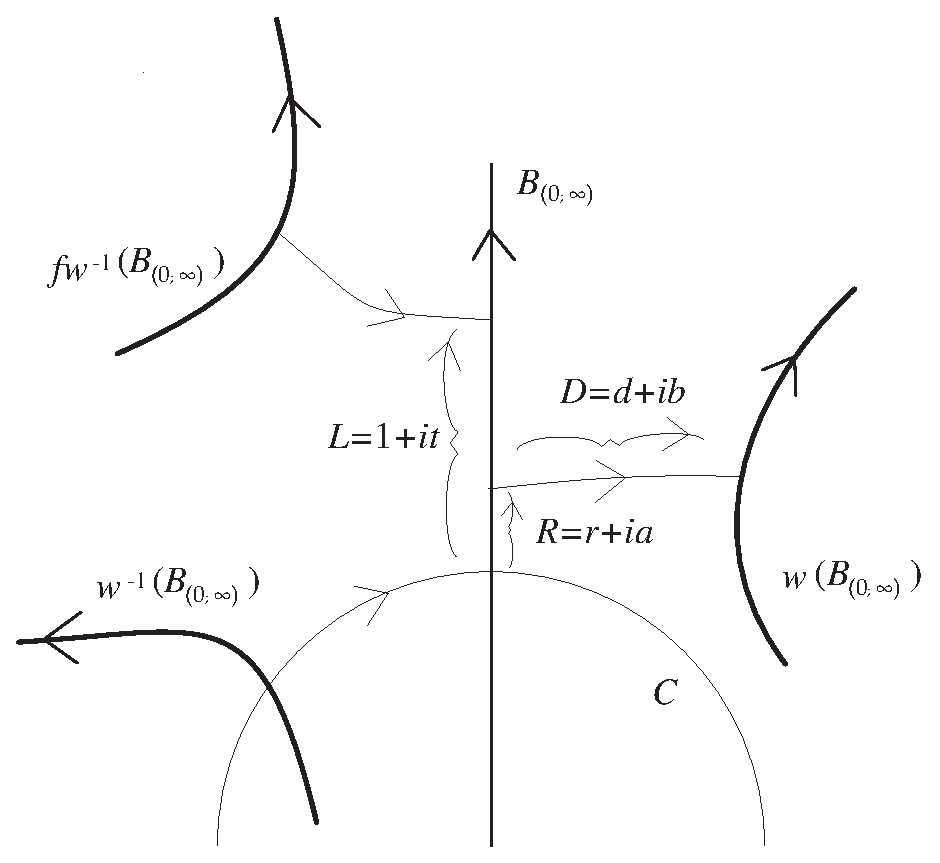
\includegraphics[scale=0.500]{fig1.1}
\end{figure}

\begin{proposition}\label{GMT prop1.10} All closed geodesics of length less than $0.0979$ in
all hyperbolic $3$\/{\textrm -}\/manifolds have {\textrm (}\/embedded\/{\textrm )} tubes of
radius $\ln(3)/2.$
\end{proposition}

\begin{proof}   In  \cite{Me} it is proved that a closed geodesic of length $x + iy$ has a tube (embedded) of radius $r(x + iy)$ satisfying 
$$
\sinh^2(r(x + iy))  =  \max_{n \in \mathbf {Z_+}} {1 \over 2} \left({\sqrt{1 - 2k(x,y,n)} \over k(x,y,n)} - 1\right) 
$$
where
$$k(x,y,n)  =  \cosh(nx) -
\cos(ny),
$$
 where we restrict to $x+iy$ values which produce positive radii $r(x + iy)$ by means of this formula. It is easy to compute that for a
given $x+iy$ we need to have $n$ for which $0 < k(x,y,n) < \sqrt 2 - 1$ to produce a positive radius tube by this method.

The function ${1 \over 2} ({\sqrt{1 - 2k} \over k} - 1)$ is decreasing on the interval $(0, -1 + \sqrt 2).$  It is easy to solve for the $k$ value that produces radius $r = \ln(3)/2$ and it is just over $0.3397.$ Thus, by restricting to $k$ values in the interval $(0,0.3397)$ we guarantee radii $r$ greater than $\ln(3)/2.$

Thus, to complete the proof of this proposition, we need to show that when a closed geodesic has real length $x$ less than 0.0979,  there exists a positive integer $n$ for which $k(x,y,n)$ is less than 0.3397
for all angles $y$.
Because $\cosh$ is an increasing function, we can restrict our analysis to $x = 0.0979.$  Thus,  we need only show that given
\pagebreak any angle $y$, we can find a positive integer $n$ such that 
$\cosh(n 0.0979) - \cos(ny) < 0.3397.$  When $n > 8$ we can compute that $\cosh(n 0.0979) - \cos(ny) > 0.3397,$ and we therefore restrict to positive integers $n \leq 8.$  

We now consider angles $y$.  Because $\cos$ is an even function, we need only consider $y \in [0, \pi].$  
Finally, we complete the proof by covering $[0,\pi]$ by 11 overlapping closed sub-intervals $\sigma_i$ each of which has an associated positive integer $n_i$ for which $\cosh(n_i 0.0979) - \cos(n_i y) < 0.3397$ is
 true for all $y \in \sigma_i$:
$$
\begin{array}{rlrlrlrl}
\sigma_0&\hskip-6pt= [0.000, 0.843] &\quad n_0 &\hskip-6pt= 1&\quad
   \sigma_5&\hskip-6pt= [1.733, 1.858] &\quad n_5 &\hskip-6pt= 7\\
 \sigma_1 &\hskip-6pt= [0.835, 0.960] & n_1&\hskip-6pt= 7&
   \sigma_6&\hskip-6pt= [1.832, 2.357] & n_6&\hskip-6pt= 3\\
 \sigma_2&\hskip-6pt= [0.951, 1.143]& n_2&\hskip-6pt= 6&
   \sigma_7&\hskip-6pt= [2.334, 2.3792]& n_7&\hskip-6pt= 8\\
 \sigma_3 &\hskip-6pt= [1.123, 1.391] & n_3&\hskip-6pt= 5&
   \sigma_8&\hskip-6pt= [2.3789, 2.647] & n_8 &\hskip-6pt= 5\\
 \sigma_4&\hskip-6pt= [1.386, 1.755] & n_4 &\hskip-6pt= 4&
   \sigma_9 &\hskip-6pt= [2.630, 2.755]&n_9&\hskip-6pt= 7\\
\end{array}
$$
\hfill $ \sigma_{10}  = [2.730, \pi] \quad  n_{10}  = 2$ 
\end{proof}

\begin{proposition}\label{GMT prop1.11} A {\textrm shortest}  geodesic $\delta$ in a closed hyperbolic $3$\/{\textrm -}\/manifold has 
\vglue4pt
{\textrm i)}  $\mathrm {tuberadius}(\delta) \ge l/4$ where $l = \Relength(\delta),$  and
\vglue4pt
{\textrm ii)} $\mathrm {tuberadius}(\delta) > \ln(3)/2$ if 
$\Relength(\delta) \ge 1.289785.$ 
\end{proposition}

\begin{proof} Part i) is a consequence of the following 
well-known argument:
Uniformly expand a tube around a shortest geodesic in the hyperbolic
$3$-manifold. 
If the expanding tube hits itself before a
radius of $l/4$ then we will construct a loop of length less than $l$, which produces a
contradiction to being shortest.  Drop the two obvious perpendiculars from
the hitting point down to the core geodesic. 
Consider the following loop---down one perpendicular, 
follow the shorter direction on the core geodesic,
up the other perpendicular. Because a lift of this loop
to $\mathbf {H}^3$ is not closed, this loop is homotopically nontrivial.  By
construction it has length less than $l/4 + l/2 + l/4 = l.$  

To prove part ii), we improve on this loop.  
Replace the first half of the journey by the
hypotenuse of the right triangle formed by the first perpendicular and the
first half of the shorter arc along the core geodesic.  Replace the second
half of the journey by the hypotenuse of the right triangle formed by the
second perpendicular and the second half of the shorter arc along the core
geodesic.  
Now, to analyze the specific case of tuberadius $\ln(3)/2$, we use
the hyperbolic Pythagorean theorem (see \cite{F}) 
$\cosh c = (\cosh a)
( \cosh b)$ with $a = \ln(3)/2$ and $b = l/4.$ 
We get that the length of the
constructed loop is $2 \Arccosh (\cosh(\ln(3)/2) \cosh (l/4))$ and this is
less than $l$ when $l > 1.289784\ldots$, 
by a calculation (which follows) and the fact that $$2 \Arccosh (\cosh(\ln(3)/2) (\cosh (l/4)) - l$$ is a decreasing function of $l$.

We solve explicitly for the value of $l$ at which
$$2 \Arccosh (\cosh(\ln(3)/2) (\cosh (l/4)) - l = 0.$$  Noting that
$\cosh(\ln(3)/2) = {2 \over \sqrt 3}$ we get ${2 \over \sqrt 3}(\cosh (l/4)) 
= \cosh(l/2).$  Using a half-angle formula for $\cosh(l/2)$ we get ${2
\over \sqrt 3}(\cosh (l/4))  = 2\cosh^2(l/4) - 1.$  Setting $x =
\cosh(l/4)$ we get the quadratic ${2 \over \sqrt 3} x = 2 x^2 -1.$
Solving and substituting, we get $l = 1.289784\ldots$ \end{proof}
\begin{definition}\label{GMT 1.12}
%\hglue-8pt 
Let $\mathcal {P}\subset\mathcal {P}^{\prime}$ be the set of those parameters $\alpha
= (l+it$, $d+ib, r+ia)$ such
that
 \vglue3pt
 a)       $0.0978\le l \le 1.289785$,
\vglue2pt b)\enspace      $l/2 \le d\le \ln(3)$,
\vglue2pt c) \enspace   $0\le r \le l/2$,
\vglue2pt d) \enspace      $-\pi \le t \le 0$,
\vglue2pt e) \enspace	$-\pi \le b \le \pi$,
\vglue2pt f) \enspace	$-\pi \le a \le \pi$.
\vglue2pt\noindent 
Define $\mathcal {T}=\mathcal {T}^{\prime}\cap \mathcal {P}.$
\end{definition}

The point of the definition of $\mathcal {P}$ and $\mathcal {T}$ is as follows.  We want to analyze by computer the relationship between lengths of shortest geodesics  and their tuberadii in hyperbolic $3$-manifolds.  We were naturally led to the parameter space 
$\mathcal {P}^{\prime}$ and its subset $\mathcal {T}^{\prime}.$  But 
$\mathcal {P}^{\prime}$ is problematic from the computational viewpoint because it is noncompact.  We wish to replace 
$\mathcal {P}^{\prime}$ by $\mathcal {P}$ which is compact, and 
$\mathcal {T}^{\prime}$ by $\mathcal {T}$ in our computer analysis.  This is carried out in Lemma \ref{GMT 1.13}.  Note that we worked to make $\mathcal {P}$ as small as reasonable to save computation time;  for example, the $t$ and $r$ restrictions above cut down the parameter space by a factor of 4 over the obvious $t$ and $r$ restrictions. 

\begin{lemma}\label{GMT 1.13}
If $\alpha=(l+it, d+ib, r+ia)\in \mathcal {T}^{\prime}$ has $d\le \ln(3)$ and
corresponds to a $2$\/{\textrm -}\/generator group
$\{G_\alpha,f_\alpha,w_\alpha\},$ then there exists a parameter $\beta=(l^{\prime}+it^{\prime}, d^{\prime}+ib^{\prime}, r^{\prime}+ia^{\prime})\in \mathcal {T}$ 
with associated group $\{G_\beta,f_\beta, w_\beta\}$ such that $G_\beta$ is conjugate (in ${\textrm Isom}(\mathbf {H}^3$)) to $G_\alpha.$ 
\end{lemma}

\begin{proof} We note that $d < l/2$ is eliminated from consideration by
Proposition \ref{GMT prop1.11}i)
and the definition of $\mathcal {T}^\prime.$ If $d\le \ln(3),$
then
$0.0978\le l\le 1.289785$ by
Propositions \ref{GMT prop1.10} and \ref{GMT prop1.11} ii)
If for the marked group $\{G, f, w\}$ we have 
$-l/2<r<0,$ then the marked group
$\{G,f,w^{-1}\}$ is conjugate to an element of $\mathcal {T}$ whose new
$r$-parameter is $-r.$  Thus we can assume that
conditions a, b, c from Definition \ref{GMT 1.12} hold for the relevant $\{G,f,w\}.$  Further,    conditions e and f hold.

This leaves condition \ref{GMT 1.12} d.  Conjugating $G$ by a
reflection in the geodesic plane spanned
by $B_{(0;\infty)}$ and $B_{(-1;1)}$ changes the $t$-parameter to 
$-t \ ({\textrm mod}\ 2\pi)$
but leaves the $r$ and $d$ parameters unchanged.
The effect on $b$ and $a$ is irrelevant.  \end{proof}

By \cite{G} Lemma 5.9
a closed orientable hyperbolic $3$-manifold $N$
satisfies the insulator condition provided that
tuberadius$(\delta) > \ln(3)/2$ for some closed geodesic $\delta\subset N.$  Thus we
are led to consider:

\begin{problem}\label{GMT 1.14}
List all closed orientable hyperbolic $3$-manifolds $N$
possessing a shortest geodesic $\delta$ such that tuberadius$(\delta)\le \ln(3)/2.$
\end{problem}

\begin{remark}\label{GMT 1.15}
If a shortest geodesic $\delta$ in $N$ satisfies tuberadius$(\delta)\le
\ln(3)/2,$ then $N$ gives
rise to an element $\alpha\in \mathcal {T}.$  (In fact $N$ may give rise to finitely many different elements of $\mathcal {T}.$)  
Thus we need to investigate:
\end{remark}

\begin{problem}\label{GMT 1.16}
Find all parameters $\alpha=(l+it, d+ib, r+ia) \in \mathcal {T}.$ 
\end{problem}

\begin{remark}\label{GMT 1.17}
	In the next     paragraphs, we will describe our method of (partially) answering Problem \ref{GMT 1.16}.  But before starting this description, we
	mention a technical point: starting with Definition \ref{GMT 1.22}, we 
will realize major advantages by working in the space $\mathcal {W} \supset \exp(\mathcal {P}),$ and
our results will ultimately be described in terms of $\mathcal {W}.$ But for now, for simplicity,  we will describe the results in terms of the unexponentiated space $\mathcal {P}.$

We will partition $\mathcal {P}$ into about one billion regions
$\{ \mathcal {P}_i\}$ and show that $\mathcal {T}$ is disjoint from all but seven small such regions.   Suppose that
$\mathcal {P}_i$ is a region of this partition and $\alpha\in \mathcal {P}_i.$  Let $h$ be a word in the
letters $f,w$ and their inverses.  Associated to the parameter
$\alpha=(l_\alpha+it_\alpha, d_\alpha+ib_\alpha, r_\alpha
+ia_\alpha)$ there are the group elements
$f_\alpha, w_\alpha$ and hence $h_\alpha.$ 
If $h_\alpha$ is not the identity then we ask
\begin{itemize}
\item[a)]  Is $\Relength (h_\alpha) < \Relength(f_\alpha) = l_\alpha?$

\item[b)]  Is Redistance$(h_\alpha(B_{(0;\infty)}), B_{(0;\infty)}) < $ Redistance$(w_\alpha(B_{(0;\infty)})$, $B_{(0;\infty)})\break = d_\alpha?$
\end{itemize}
\noindent If either a) or b) is true, then $\alpha\notin \mathcal {T}.$

Now let $\beta\in \mathcal {P}_i,$
with $f_\beta, w_\beta,$ and $h_\beta$ the associated hyperbolic isometries.  If
say a) is true for $\alpha$
then so is the statement $\Relength(h_\beta) < \Relength(f_\beta)\break = l_\beta$ for
$\beta$ sufficiently close to $\alpha.$
Thus we can show that $\mathcal {T}\cap \mathcal {P}_i =\emptyset$ if we can find an $\alpha$ for
which, say, statement a) is true, and then
use first-order Taylor approximation (with error/remainder term) to show that the corresponding
statement holds for all $\beta\in \mathcal {P}_i $ while continuing to avoid the prohibition that $h_\beta$ not be the identity.
\end{remark}


\begin{definition}  \label{GMT 1.18} A word $h$ in $w,f,w^{-1},f^{-1}$ for which statement a) (resp.\ b)) in
Remark \ref{GMT 1.17}
holds for each $\beta\in \mathcal {P}_i$
and for which $h_\beta$ is not a power of $f_\beta$ for each $\beta\in \mathcal {P}_i$ is
called a {\textit killerword} for $\mathcal {P}_i$ with respect to contradiction a) (resp.\ b)).
\end{definition}

\begin{summary}  \label{GMT 1.19} With seven exceptions,  to each of the approximately one
billion regions partitioning $\mathcal {P},$ we will
associate a killerword and a contradiction.  \end{summary} 

\begin{remark}  \label{GMT 1.20} Computers are well suited for partitioning a set such as $\mathcal {P}$
into many regions $\{ \mathcal {P}_i \},$ and finding a
killerword $h_i$ which eliminates all $\alpha_i \in \mathcal {P}_i $ due to contradiction $C_i.$
Depending on the contradiction, we find
computable expressions  for approximations of the values of
$\Relength(h_\beta)$ or Redistance$(h_\beta(B_{(0;\infty)}), B_{(0;\infty)})$ and
thus use the computer to eliminate all of~$\mathcal {P}_i .$ 
\end{remark}

\begin{remark}\label{GMT 1.21}.
	To analyze Relength and Redistance as in Remark \ref{GMT 1.17}, we would be led to work with the $\Arccosh$ function, because, 
$$\mathrm {length}(f) = 2\Arccosh(\mathrm {trace}(A)/2)$$
where $A\in \mathrm {SL}(2,\mathbf {C})$ represents the isometry $f.$
(As we do not need this formula for $\mathrm {length}(f)$ we will neither prove the formula, nor explain technical details about it.)  This would be problematic from the view-point of error analysis---we do not want to deal with transcendental functions such as $\Arccosh.$  

This problem can be  avoided slickly by exponentiating the preliminary parameter space $\mathcal {P}$ to get the parameter space $\mathcal {W}$ (the
	definition of $\mathcal {W}$ is given in Definition \ref{GMT 1.22}).   Lemmas \ref{GMT 1.24} and \ref{GMT 1.25} then demonstrate
that while working in $\mathcal {W}$ one need only
understand the basic arithmetic operations $+, -, \times, /, \sqrt{}$.
The machine implementation of these basic operations is governed by the IEEE standard IEEE-754 (see \cite{IEEE}).
\end{remark}
\vglue8pt

To expand a bit on the problematic nature of transcendental 
functions, we note that
our computer version of Taylor approximations (see Preview \ref{GMT 1.35} and
Chapters \ref{Ch.AffApprox} and \ref{Ch.AffWithEPS}
) is designed to work for functions built up out of the basic arithmetic operations.  It would be a nightmare to include
functions such as the Arccosh.
\vglue8pt 
\begin{definition} \label{GMT 1.22} Let 
\vglue4pt
\centerline{$ \mathcal {W} = \{ (x_0,x_1,x_2,x_3,x_4,x_5) : |x_i| \le 4 \times 2^{(5 - i) /6} \mathrm {\ for\ } i = 0,1,2,3,4,5 \}$}
\begin{eqnarray*}
\noalign{\vskip-12pt}
 \supset \exp(\mathcal {P}) = 
\{(x_0,x_1,x_2,x_3,x_4,x_5)\mid \hskip-16pt&\hskip-16pt & 
x_0 + i x_3=\exp(e),  \enspace x_1 + i x_4
  = \exp(f),  \\
\hskip-16pt&\hskip-16pt& x_2 + i x_5 = \exp(g) \
{\textrm where} (e,f,g)\in \mathcal {P}\}\\
\noalign{\vskip-28pt}
\end{eqnarray*}
 and let
$$\mathcal {S}=\exp(\mathcal {T}).$$
As we are taking $\exp$ of the various complex co-ordinates, it is notationally convenient to replace our complex parameters 
$L = l+it,\ D = d+ib,\ R = r+ia$ by exponentiated versions.  That is, let 
\begin{eqnarray*}
L^\prime &\hskip-8pt=\hskip-8pt& \exp(L) = \exp(l+it),\enspace D^\prime = \exp(D) = \exp(d + ib), 
\\ R^\prime &\hskip-8pt=\hskip-8pt& \exp(R) = \exp(r+ia).
\end{eqnarray*}\end{definition}
 

\begin{remarks}\label{GMT 1.23}
i) We work with $\mathcal {W}$ instead of $\exp(\mathcal {P})$ because we want our initial parameter space to be a (6-dimensional) box that is easily
subdivided.  This has the side effect that certain regions (sub-boxes)
 $\mathcal {W}_i$ of $\mathcal {W}$ will be eliminated because they are outside of $\exp(\mathcal {P})$ not because of the analogues of conditions a) and b) in
Remark \ref{GMT 1.17}
	The entire collection of conditions is given in Chapter \ref{Ch.ConditionsTree}.
 
ii)  The presence of the factor $2^{(5-i)/6}$ in the definition of $\mathcal {W}$ is explained in Construction \ref{GMT 5.3}.
Briefly, the main reason for including it
is to make the shape of regions stay as uniform and ``round" as possible under subdivision.
This makes the Taylor approximations efficient, hence fast.
\vglue4pt
iii)  We chose the co-ordinates of $\mathcal {W}$  so that $L^\prime = x_0 + i x_3,\ D^\prime = x_1 + i x_4,\ R^\prime = x_2 + i x_5\ $ to gain a mild
computer advantage.  \end{remarks}

\begin{lemma}\label{GMT 1.24}  If $(L^\prime, D^\prime, R^\prime)\in \mathcal {W}$ and  $\{G,f,w\}$ is the associated normalized 
marked group{\textrm ,} then $f$ and $w$ have matrix representatives
 $$ f = \left(
	\begin{matrix}
		\sqrt{L^\prime}&0\cr
		0 & 1/\sqrt{L^\prime}\cr
	\end{matrix}
	\right), \leqno\mathrm{ a)}$$

	$$ w = \left(\begin{matrix}
		\sqrt{R^\prime} * ch & \sqrt{R^\prime} * sh \cr
		sh / \sqrt{R^\prime} & ch/\sqrt{R^\prime}\cr
	\end{matrix}
	\right) \leqno\mathrm {b)}$$ 
where 
$ch = (\sqrt{D^\prime} + 1/\sqrt{D^\prime})/2\ \ {\textrm and}\ \ 
sh = (\sqrt{D^\prime} - 1/\sqrt{D^\prime})/2.$
\end{lemma}
 
\begin{proof}{}  a)  In our set-up  the (oriented) axis of $f$ is $B_{(0;\infty)}$.  
As such, $f$ corresponds to a diagonal matrix, with diagonal entries $p$ and $p^{-1},$  with $|p| >1.$ 
The action of $f$ on the bounding complex plane is simply multiplication by $p^2.$  Extending this action to upper-half-space in the natural way rotates the $z$-axis by angle $\arg(p^2)$ and sends $(0,0,1)$ to $(0,0,|p|^2).$ 
 Thus, $$\mathrm {Im}(\length(f)) = \arg(p^2) = \mathrm {Im}(\ln(p^2))$$ and,
using the hyperbolic metric, 
$$\mathrm {Re}(\length(f)) = \ln(|p|^2) = \mathrm {Re}(\ln(p^2)).$$
That is, $\length(f) = \ln(p^2)$ and 
$$p = \pm \exp(\length(f)/2) = \pm \sqrt{\exp(\length(f))} = \pm \sqrt{\exp(L)} = \pm \sqrt{L^\prime}.$$ Now, we take the positive square
root (taking the negative square root produces the other lift from 
${\textrm PSL(2,}\mathbf {C})$ to $\mathrm {SL(2,}\mathbf {C})$).

b)  $w = \beta \circ \alpha$ where $\beta$ is translation of distance $R$ along $ B_{(0;\infty)}$ and $\alpha$ is translation of distance $D$ along $ B_{(-1;1)}$.  Thus,
	a matrix representative of $\beta$ is $$ \left(\begin{matrix}\sqrt{R^\prime} & 0 \cr 0 & 1/\sqrt{R^\prime}\cr\end{matrix}\right)$$ and a matrix representative of $\alpha$ can be computed to be $$\left(\begin{matrix}\cosh(D/2) & \sinh(D/2) \cr \sinh(D/2) & \cosh(D/2)\cr\end{matrix}\right).$$ But
$\cosh(D/2) = (\exp(D/2) + \exp(-D/2))/2 = 
(\sqrt{D^\prime} + 1/\sqrt{D^\prime})/2 = ch$ and similarly for $sh.$
Thus, $$\alpha = \left(\begin{matrix}ch & sh \cr sh & ch\cr\end{matrix}\right)$$ and b) follows by matrix multiplication.
\end{proof}

\begin{lemma}\label{GMT 1.25} If $h \in {\textrm Isom}_+(\mathbf {H}^3)$ is represented by the matrix $$A = \left(\begin{matrix}a &  b \cr c & d\cr\end{matrix}\right)\in \mathrm {SL}(2,\mathbf {C}),$$ then 
\begin{itemize}
\item{a)} $\exp(\Relength (h))= |\trace(A)/2 \pm \sqrt{(\trace(A)/2)^2 - 1}|^2,$

\item{b)} $\exp({\textrm Redistance} (h(B_{(0;\infty)}), B_{(0;\infty)}))=|{\textrm orthotrace}(A) \pm$\hfill \noindent $\sqrt{(\mathrm {orthotrace}(A))^2 - 1}|$  where 
{\textrm orthotrace(}$A) = ad + bc.$ $\phantom{\sum^\int}$
\end{itemize}
In both cases{\textrm ,} the $+, -$ produce reciprocal values for the right\/{\textrm -}\/hand side{\textrm ,}
  and we take the one producing the larger value{\textrm ,} unless the value is $1${\textrm ,} in
which case there is no need to choose.
\end{lemma}

\begin{proof}{}  a)  If $A$ is elliptic or parabolic, the proof is straightforward (the trace of a parabolic is $\pm 2$ while the trace of an elliptic
is a real number between 2 and -2).  

We assume $A$ is hyperbolic.  Because trace is a conjugacy invariant, we can assume the oriented axis of $A$ is $ B_{(0;\infty)}.$  Thus $A$ is a diagonal matrix with $p$ and $p^{-1}$ along the diagonal with 
$|p| > 1,$ and, as in the proof of Lemma \ref{GMT 1.24}, we see that 
$\exp({\textrm length}(h)) = p^2.$  Of course,  $\trace(A)= p + p^{-1}$, and it is easy enough to solve for $p.$   Specifically, 
$p = \trace(A)/2 \pm \sqrt{(\trace(A)/2)^2 - 1}.$
Thus, 
\begin{eqnarray*}
\exp(\Relength (h))& =& |\exp(\length(h))|  = 
|p|^2\\[5pt]
&=& |(\trace(A)/2) \pm \sqrt{(\trace(A)/2)^2 - 1}|^2.
\end{eqnarray*}
\vglue4pt
b)  If $ B_{(0;\infty)}$ and $h(B_{(0;\infty)})$ intersect at infinity, then the proof is straightforward.  For example, 
if $h$ fixes the point $(0,0,0)$ at infinity, then $c = 0,\ ad = 1$ and the formula holds.  Similarly for the other cases in which $ B_{(0;\infty)}$ and $h(B_{(0;\infty)})$ intersect at infinity.

We assume $ B_{(0;\infty)}$ and $h(B_{(0;\infty)})$ do not intersect at infinity. We will compute the length of $k$, the square of the transformation taking $ B_{(0;\infty)}$ to $h(B_{(0;\infty)})$ along their ortholine. 
Let $\tau$ be 180-degree rotation about $ B_{(0;\infty)},$ then $(h \circ \tau \circ h^{-1})$ is 180-degree rotation about $h(B_{(0;\infty)}),$ and
we have that  $k = (h \circ \tau \circ h^{-1}) \circ \tau.$   
Now, $\tau$ and $h$ are represented by the matrices 
$$ \left(\begin{matrix} i & 0 \cr 
0  & -i \cr\end{matrix} \right) \mathrm {\ \ and\ \ } 
                         \left(\begin{matrix} a & b \cr 
			 c  & d \cr\end{matrix} \right)  \in \mathrm {SL}(2,\mathbf {C}).$$ 
Hence,   $k = (h \circ \tau \circ h^{-1}) \circ \tau$ can be computed to have matrix
representation $$\left(\begin{matrix} ad + bc & 2ab \cr 
2cd & ad + bc \cr\end{matrix} \right).$$ 
Thus,
\begin{eqnarray*}
&&\hskip-66pt\exp({\textrm Redistance} (h(B_{(0;\infty)}), B_{(0;\infty)}))\\
& = &
\exp(\Relength(k)/2)= \sqrt{|\exp(\length(k)|}\\
& =&
|(\trace(k)/2) \pm \sqrt{(\trace(k)/2)^2 - 1}|\\
& =&
|(ad + bc) \pm \sqrt{(ad + bc)^2 - 1}|. \\
\noalign{\vskip-36pt}
\end{eqnarray*}
\end{proof}

\begin{remark}\label{GMT 1.26} i)  It follows from Lemma \ref{GMT 1.25} that if $h$ is a word in $f,w,f^{-1},w^{-1},$ then for any
parameter value $\alpha\in \mathcal {W},$
$$\exp(\Relength(h_\alpha)), \hbox{ and }
  \exp({\textrm Redistance}(h_\alpha(B_{(0;\infty)}), B_{(0;\infty)}))$$ can be computed using only the
operations $+, -, \times, /, \sqrt{}.$
\vglue4pt

 ii) During the course of the computer work needed to prove the main theorems, the parameter space
$\mathcal {W}$ was decomposed into sub-boxes by computer via a recursive subdivision process:
Given a sub-box  being analyzed, either it can be {\textit killed directly} (that is, eliminated by a killerword and associated condition as described in
Remark \ref{GMT 1.17}
or for the trivial reason described in Remark \ref{GMT 1.23} i), or it cannot.  
If it cannot be killed directly, it is subdivided in half by a hyperplane
$\{x_i = c \}$ (where $i$ runs through the various co-ordinate dimensions
cyclically) and the two pieces are analyzed separately, and so on. 

As such, a sub-box of $\mathcal {W}$ can be described by a sequence of 0's and 1's where 0 means ``take the lesser $x_i$ values" and 1 means ``take the greater $x_i$ values."  
For the decomposition of $\mathcal {W}$ into sub-boxes, all the 
sub-box descriptions could be neatly encoded into one tree (although in practice we found it preferable to use several trees to describe the entire
	decomposition.  See Chapter \ref{Ch.ConditionsTree}).
\vglue4pt
iii) In the following proposition, seven {\textit exceptional boxes} are described as sequences of 0's and 1's.  
Four of the exceptional boxes---$X_0, X_4, X_5, X_6$---are each the union of two abutting sub-boxes, $X_0 = X_{0a} \cup X_{0b}$ and so on.  It is a pleasant exercise to work through the fact that they abut.  
It should be noted that had the set-up for $\mathcal {W}$ been different, more sub-boxes (or perhaps fewer) might have been needed to construct the seven
exceptional regions. 

It is also a pleasant exercise to calculate by hand the co-ordinate ranges of the various sub-boxes.  For example, the range of the last co-ordinate (i.e., $x_5$) of the sub-box 
\eject

\noindent 
$X_{6a} = 
111000000001000111\ 
111111110101001111\ 
011111010111111111$\hfill
\vglue4pt
  \hfill $  
110001001011000111\ 0$
\vglue4pt\noindent 
is found by taking the 6th entry, the 12th entry, the 18th entry, and so on.  These entries are 011111111111.  The first entry (0) means take the
lesser $x_5$ values, and produces the interval $[-4,0].$  The second entry (1) means take the greater $x_5$ values, and produces the interval
$[-2,0].$  The third entry (1) produces $[-1,0].$  Continuing, we see that $X_{6a}^{\phantom{|}}$ has $-2^{-9} \le x_5 = \mathrm {Im}(R') \le 0.$  The other
co-ordinates can be computed in the same fashion, although they must at the end be multiplied by the factor $2^{(5 - i)/6}$ (see the definition of the
initial box
$\mathcal {W}$).  The range of co-ordinate values for each  exceptional  box $X_0, X_1, \ldots, X_6$ is given in Table \ref{GMT tab 1.1} (a limited number of significant
digits is given), and  then a range of co-ordinates for exceptional regions (in $\mathcal {P}$) 
$\mathcal {R}_i \supset \exp^{-1}(X_i)$ is given (see
Remarks \ref{GMT 1.30}i) and \ref{GMT 1.30}ii)
in Table \ref{GMT tab 1.2}. (Note that this use of the symbol $\mathcal {R}_i$ differs
slightly from the use in \S 0.)
Finally, two {\textit quasi-relators} are given in Theorem \ref{GMT 1.28} for each exceptional box $X_0, X_1, \ldots, X_6$ (see the next definition).\end{remark}
 
\begin{definition} \label{GMT 1.27} A {\textit quasi-relator} in a sub-box $X$ of $\mathcal {W}$ is a word in $f,w,F=f^{-1},W=w^{-1}$ that is close to the identity
throughout
$X$ and experimentally appears to be converging to the identity at some point in $X.$  In particular, a quasi-relator rigorously has Relength less than
that of $f$ at all points in $X.$
\end{definition}

\begin{theorem}\ref{GMT 1.28}  
Within the parameter space $\mathcal {W}$ but outside the seven exceptional boxes there are no parameter points corresponding to 
marked groups $\{G,f,w\}$ where $G$ is 
discrete{\textrm ,} torsion\/{\textrm -}\/free and  parabolic\/{\textrm -}\/free\/{\textrm ;}
$f$ corresponds to a shortest geodesic $\delta$ of tuberadius $\le
\ln(3)/2${\textrm ;} and $w$ takes a particular lift of $\delta$ to 
a nearest translate.
 Specifically{\textrm ,} 
$\mathcal {S} \cap (\mathcal {W} - \bigcup_{n = 0,\dots, 6} X_n)=\emptyset$ where the $X_n$ are the exceptional boxes

\vglue4pt

 \noindent $X_0 = X_{0a} \cup X_{0b},$
\vglue8pt
\noindent $X_{0a} = 
001000110111110001\ 
101001010101011001\ 
011011010111101101$\hfill 

 
 \hfill
$100001101101000111\ 
010001110101100101\ 
1101110111110100,$  
\vglue8pt
 \noindent $X_{0b} = 
001001110110110000\ 
101000010100011000\ 
011010010110101100$

\hfill
$100000101100000110\ 
010000110100100100\ 
1101100111100100,$ 
 \vglue4pt
\noindent  $X_0\ \ $ quasi\/{\textrm -}\/relators\/{\textrm :}

$r_1 = fwFwwFwfww,$
 
$r_2 = FwfwfWfwfw,$

\vglue8pt
\noindent $X_1 = 
001000110001110110\ 
011101000110111110\ 
100010110000100011$\hfill 

\hfill $
101101001101001000\ 
110101011000000100\ 
000.$ 

\noindent $X_1\ \ 
$ quasi\/{\textrm -}\/relators\/{\textrm :}

$r_1 = FFwFWFWfWFWFwFFww,$
 
$r_2 = FFwwFwfwfWfwfwFww,$
\vglue4pt
\noindent $X_2 = 
001000110101010010\ 
101010110001100101\ 
110111100001101010$\hfill

\hfill $111100100000010001\ 
111100,$
\vglue4pt
\noindent $X_2\ \ $ quasi\/{\textrm -}\/relators\/{\textrm :}

$r_1 = FwfwfWffWfwfwFww,$

$r_2 = FFwFFwwFwfwfwFww,$
\vglue4pt
\noindent 
$X_3 = 
111000000001000110\ 
011011101101011000\ 
111101011110001100$\hfill

\hfill  
$111111100110110000\ 
0000100010100010,$
\vglue4pt
\noindent $X_3\ \ $ quasi\/{\textrm -}\/relators\/{\textrm :}\/

$r_1 = FFwfwFFwwFWFwFWfWFWffWFWfWFwFWFww,$ 

$r_2 = FFwfwFwfWfwfWWfwfWfwFwfwFFwwFWFww,$
\vglue4pt 
\noindent $X_4 = X_{4a} \cup X_{4b},$
\vglue4pt
\noindent $X_{4a} = 
111000000001000110\ 
011001001111101010\ 
011110110110111101$\hfill

\hfill  
$100011111110110110\ 
10000111101,$
\vglue4pt
\noindent $X_{4b} = 
111000000001000110\ 
011001001111101010\ 
111110010110011101$\hfill

\hfill  
$000011011110010110\ 
00000101101,$
\vglue4pt
\noindent $X_4\ \ $ quasi\/{\textrm -}\/relators\/{\textrm :}

$r_1 = FFwfwFwfWfwfWfwFwfwFFwwFWFwFWFww,$

$r_2 = FFwfwFwfwFFwwFWFwFWfWFWfWFwFWFww,$
\vglue4pt
\noindent $X_5 = X_{5a} \cup X_{5b},$
\vglue4pt
\noindent $X_{5a} = 
001000110001110111\ 
001111000101111111\ 
101111100111001111$\hfill

\hfill 
$000001111011110111\ 1,$
\vglue4pt
\noindent  $X_{5b} = 
001001110000110110\ 
001110000100111110\ 
101110100110001110$\hfill

\hfill  
$000000111010110110\ 1,$
\vglue4pt
\noindent $X_5\ \ $ quasi\/{\textrm -}\/relators\/{\textrm :}

$r_1 = FwFWFwFwfwfWfwfw,$

$r_2 = FwfwfWfWFWfWfwfw,$
\vfil
\noindent $X_6 = X_{6a} \cup X_{6b},$
\vfil
\noindent $X_{6a} = 
111000000001000111\ 
111111110101001111\ 
011111010111111111$\hfill

\hfill  
$110001001011000111\ 0,$
\vglue4pt

\noindent $X_{6b} = 
111001000000000110\ 
111110110100001110\ 
011110010110111110$\hfill

\hfill  
$110000001010000110\ 0,$
\vglue4pt
\noindent $X_6\ \ $ quasi\/{\textrm -}\/relators\/{\textrm :}\/

$r_1 = FWFwFWfWFwFWFwfw,$

$r_2 = FWFwfwFwfWfwFwfw.$
\end{theorem}

 
\begin{proof}{}  
The proof follows along the lines presented in
Remark \ref{GMT 1.17}
Two computer files contain the data needed for the proof.   
The first computer file describes the partition of $\mathcal {W}$ into
sub-boxes and attaches an integer to each such sub-box, 
and the second file, called ``conditionlist" is an ordered list of conditions and killerwords.
The integer associated to a sub-box in the first file describes the numbered condition/killerword from   conditionlist that will eliminate the sub-box
in question (other than those corresponding to the $X_i).$ A computer program named {\textit verify} shows
that the conditions and killerwords in question actually do kill off their associated sub-boxes (see
	Section \ref{Ch.ConditionsTree}
	for more details).  This computer
program addresses the issues of Remark \ref{GMT 1.20}.  The code for {\textit
verify} is available at the {\textit Annals} web site. 

In addition, a mild modification of {\textit verify} showed that the listed words were quasi-relators for the given sub-boxes. 
\end{proof}

\begin{corollary}\label{GMT 1.29}
If $\delta$ is a shortest geodesic in $N,$ a closed orientable
hyperbolic $3$\/{\textrm -}\/manifold{\textrm ,} then 
\begin{itemize}
\item{i)}  either {\textrm tuberadius(}$\delta) > \ln(3)/2$ or
$\exp(\length(\delta))\in \mathcal {L}(X_k)$ for some\break $k\in {0,\ldots,6}$
 where $\mathcal {L}(X_k)$
denotes the range of $L^\prime$ values in the 
exceptional box $X_k.$ 

\item{ii)} Either {\textrm tuberadius(}$\delta) > \ln(3)/2$ or
${\textrm tuberadius}(\delta) = \mathrm {Re}(D)/2$ where\break $\exp(D)
\in \mathcal {D}(X_k)$ for some $k\in {0,\ldots,6}$
 and $\mathcal {D}(X_k)$
denotes the range of $D^\prime$ values in the 
exceptional box $X_k.$\hfill\qed
\end{itemize}

\end{corollary}

 
\begin{table}\label{GMT tab 1.1}
\caption{Exceptional boxes in $(L',D',R')$ co-ordinates in $\mathcal {W}$; truncated values}
 
\begin{small}
$$
\begin{array}{rlrlrlrl}
\noalign{\noindent $X_0$}
\noalign{\vskip2pt}
l'_{\textrm min} &\hskip-6pt = -0.84065&\enspace l'_{\textrm max} &\hskip-6pt = -0.84060&\enspace
t'_{\textrm min}&\hskip-6pt = -2.13726&\enspace t'_{\textrm max}&\hskip-6pt = -2.13722\\
 d'_{\textrm min}&\hskip-6pt = -0.84064& d'_{\textrm max} &\hskip-6pt = -0.84059&
b'_{\textrm min}&\hskip-6pt = -2.13729& b'_{\textrm max} &\hskip-6pt = -2.13722\\
r'_{\textrm min} &\hskip-6pt = 0.999979& r'_{\textrm max} &\hskip-6pt = 1.000022&
a'_{\textrm min}&\hskip-6pt = -0.00006103& a'_{\textrm max}&\hskip-6pt = 0.00006103\end{array}
$$
$$
\begin{array}{rlrlrlrl}
\noalign{\vskip2pt}
\noalign{ \noindent $X_1$}
\noalign{\vskip2pt}
l'_{\textrm min} &\hskip-6pt = -1.34852&\enspace  l'_{\textrm max} &\hskip-6pt = -1.34831&\enspace 
t'_{\textrm min} &\hskip-6pt = -2.66102&\enspace  t'_{\textrm max} &\hskip-6pt = -2.66072\\
d'_{\textrm min} &\hskip-6pt = -0.54334& d'_{\textrm max}
&\hskip-6pt = -0.54315&   b'_{\textrm min} &\hskip-6pt = -2.85877&  b'_{\textrm max} &\hskip-6pt = -2.85849\\
r'_{\textrm min} &\hskip-6pt = 0.90390& 
r'_{\textrm max} &\hskip-6pt = 0.90408&   a'_{\textrm min} &\hskip-6pt = -1.47167&  a'_{\textrm max} &\hskip-6pt = -1.47143
\end{array}
$$
$$
\begin{array}{rlrlrlrl}
\noalign{\vskip2pt}
\noalign{\noindent $X_2$}
\noalign{\vskip2pt}
l'_{\textrm min} &\hskip-6pt =  -1.78701&\enspace   l'_{\textrm max} &\hskip-6pt =  -1.78527&\enspace  
t'_{\textrm min} &\hskip-6pt =  -2.27253&\enspace   t'_{\textrm max} &\hskip-6pt =  -2.27130\\
d'_{\textrm min} &\hskip-6pt =  -1.07428& d'_{\textrm max}
&\hskip-6pt =  -1.07273&   b'_{\textrm min} &\hskip-6pt =  -2.71846&  b'_{\textrm max} &\hskip-6pt =  -2.71736\\
r'_{\textrm min} &\hskip-6pt =  0.74163& 
r'_{\textrm max} &\hskip-6pt =  0.74301&   a'_{\textrm min} &\hskip-6pt =  -1.52929&  a'_{\textrm max} &\hskip-6pt =  -1.52832
\end{array}
$$

$$
\begin{array}{rlrlrlrl}
\noalign{\noindent 
$X_3$}
\noalign{\vskip2pt} l'_{\textrm min} &\hskip-6pt =   0.58117&\enspace   l'_{\textrm max} &\hskip-6pt =   0.58160&\enspace  
t'_{\textrm min} &\hskip-6pt =   -3.31221&\enspace   t'_{\textrm max} &\hskip-6pt =   -3.31190\\
d'_{\textrm min} &\hskip-6pt =   1.15644& d'_{\textrm max}
&\hskip-6pt =   1.15683&  b'_{\textrm min} &\hskip-6pt =   -2.75628& b'_{\textrm max} &\hskip-6pt =   -2.75573\\
r'_{\textrm min} &\hskip-6pt =   1.40420&
r'_{\textrm max} &\hskip-6pt =   1.40454&  a'_{\textrm min} &\hskip-6pt =   -1.17968& a'_{\textrm max} &\hskip-6pt =   -1.17919
\end{array}
$$
$$
\begin{array}{rlrlrlrl}
\noalign{\noindent 
$X_4$}
\noalign{\vskip2pt}
l'_{\textrm min} &\hskip-6pt = 0.33321&\enspace   l'_{\textrm max} &\hskip-6pt = 0.33495&\enspace  
t'_{\textrm min} &\hskip-6pt = -3.31959&\enspace   t'_{\textrm max}&\hskip-6pt = -3.31898\\
d'_{\textrm min} &\hskip-6pt = 0.97739& d'_{\textrm max}
&\hskip-6pt = 0.97817&  b'_{\textrm min} &\hskip-6pt = -2.82533& b'_{\textrm max} &\hskip-6pt = -2.82478\\
r'_{\textrm min} &\hskip-6pt = 1.35413&
r'_{\textrm max} &\hskip-6pt = 1.35482&  a'_{\textrm min} &\hskip-6pt = -1.22558& a'_{\textrm max} &\hskip-6pt = -1.22460\end{array}$$
$$\begin{array}{rlrlrlrl}
\noalign{\noindent 
$X_5$}
\noalign{\vskip2pt}
l'_{\textrm min} &\hskip-6pt = -1.37984&\enspace   l'_{\textrm max}&\hskip-6pt = -1.37810&\enspace  
t'_{\textrm min} &\hskip-6pt = -2.53706&\enspace   t'_{\textrm max} &\hskip-6pt = -2.53460\\
d'_{\textrm min} &\hskip-6pt = -1.37967& d'_{\textrm max}
&\hskip-6pt = -1.37657&  b'_{\textrm min}&\hskip-6pt = -2.53650& b'_{\textrm max} &\hskip-6pt = -2.53430\\
r'_{\textrm min} &\hskip-6pt = 0.99989&
r'_{\textrm max} &\hskip-6pt = 1.00265&  a'_{\textrm min} &\hskip-6pt = -0.001953& a'_{\textrm max} &\hskip-6pt = 0.001953\end{array}$$

$$\begin{array}{rlrlrlrl}
\noalign{\noindent 
$X_6$}
\noalign{\vskip2pt}
l'_{\textrm min} &\hskip-6pt = 1.37810&\enspace   l'_{\textrm max}&\hskip-6pt = 1.37984&\enspace  
t'_{\textrm min} &\hskip-6pt = -2.53706&\enspace   t'_{\textrm max} &\hskip-6pt = -2.53460\\
d'_{\textrm min} &\hskip-6pt = 1.37657& d'_{\textrm max}
&\hskip-6pt = 1.37967& b'_{\textrm min} &\hskip-6pt = -2.53650& b'_{\textrm max}&\hskip-6pt = -2.53430\\
r'_{\textrm min} &\hskip-6pt = 0.99989&
r'_{\textrm max} &\hskip-6pt = 1.00265&  a'_{\textrm min} &\hskip-6pt = -0.001953& a'_{\textrm max} &\hskip-6pt = 0.001953
\end{array}$$
\end{small}
 \vglue12pt
 \end{table}

\begin{table}\label{GMT tab 1.2}
\caption{Exceptional regions (boxes) in $(L,D,R)$ co-ordinates in $\mathcal {P}$}
\begin{small}
$$
\begin{array}{rlrl}
\noalign{\noindent  $\mathcal {R}_0$}
\noalign{\vskip2pt}
l_{\textrm min} &\hskip-6pt =  0.8314&\enspace    l_{\textrm max}&\hskip-6pt  = 0.8315\\
t_{\textrm min} &\hskip-6pt =  -1.9456&\enspace    t_{\textrm max}&\hskip-6pt  = -1.9455\\
d_{\textrm min} &\hskip-6pt =  0.8314&  d_\mathrm {max}&\hskip-6pt  = 0.8315\\   b_{\textrm min} &\hskip-6pt =  -1.9456&  b_{\textrm max} &\hskip-6pt = -1.9455\\
r_{\textrm min} &\hskip-6pt =  -0.00002051&  r_{\textrm max} &\hskip-6pt = 0.00002267\\  a_{\textrm min} &\hskip-6pt =  -0.00006105&  a_\mathrm {max}&\hskip-6pt  = 0.00006105\end{array}
$$

%$$
%\begin{array}{rlrlrlrl}
%\noalign{\noindent  $\mathcal {R}_0$}
%\noalign{\vskip2pt}
%l_{\textrm min} &\hskip-6pt =  0.8314&\enspace    l_{\textrm max}&\hskip-6pt  = 0.8315&\enspace   
%t_{\textrm min} &\hskip-6pt =  -1.9456&\enspace    t_{\textrm max}&\hskip-6pt  = -1.9455\\
%d_{\textrm min} &\hskip-6pt =  0.8314&  d_\mathrm {max}&\hskip-6pt  = 0.8315&   b_{\textrm min} &\hskip-6pt =  -1.9456&  b_{\textrm max} &\hskip-6pt = -1.9455\\
%r_{\textrm min} &\hskip-6pt =  -0.00002051&  r_{\textrm max} &\hskip-6pt = 0.00002267&   a_{\textrm min} &\hskip-6pt =  -0.00006105&  a_\mathrm {max}&\hskip-6pt  = 0.00006105\end{array}
%$$


$$\begin{array}{rlrlrlrl}
\noalign{\noindent  $\mathcal {R}_1$}
\noalign{\vskip2pt}
l_{\textrm min} &\hskip-6pt =  1.0928&\enspace    l_{\textrm max} &\hskip-6pt = 1.0931&\enspace   
t_{\textrm min} &\hskip-6pt =  -2.0399&\enspace   t_{\textrm max}&\hskip-6pt  = -2.0397\\
d_{\textrm min} &\hskip-6pt =  1.0680&  d_\mathrm {max}&\hskip-6pt  = 1.0682&   b_{\textrm min} &\hskip-6pt =  -1.7587&  b_{\textrm max} &\hskip-6pt = -1.7585\\
r_{\textrm min} &\hskip-6pt =  0.5463& 
r_{\textrm max}&\hskip-6pt  = 0.5465&   a_{\textrm min} &\hskip-6pt =  -1.0201&  a_{\textrm max}&\hskip-6pt  = -1.0198\end{array}$$

$$\begin{array}{rlrlrlrl}\noalign{\noindent  $\mathcal {R}_2$}
\noalign{\vskip2pt}
l_{\textrm min} &\hskip-6pt =  1.0608&\enspace    l_{\textrm max} &\hskip-6pt = 1.0617&\enspace   
t_{\textrm min} &\hskip-6pt =  -2.2375&\enspace    t_{\textrm max} &\hskip-6pt = -2.2366\\
d_{\textrm min} &\hskip-6pt =  1.0720&  d_\mathrm {max}&\hskip-6pt  = 1.0727&   b_{\textrm min} &\hskip-6pt =  -1.9473&  b_{\textrm max} &\hskip-6pt = -1.9466\\
r_{\textrm min} &\hskip-6pt =  0.5298& 
r_{\textrm max} &\hskip-6pt = 0.5308&   a_{\textrm min} &\hskip-6pt =  -1.1193&  a_{\textrm max} &\hskip-6pt = -1.1182\end{array}$$

$$\begin{array}{rlrlrlrl}
\noalign{\noindent  $\mathcal {R}_3$}
\noalign{\vskip2pt}
l_{\textrm min} &\hskip-6pt =  1.2126&\enspace    l_{\textrm max} &\hskip-6pt = 1.2129&\enspace   
t_{\textrm min} &\hskip-6pt =  -1.3972&\enspace    t_{\textrm max}&\hskip-6pt  = -1.3969\\
d_{\textrm min} &\hskip-6pt =  1.0947&  d_\mathrm {max}&\hskip-6pt  = 1.0951&   b_{\textrm min} &\hskip-6pt =  -1.1736&  b_{\textrm max}&\hskip-6pt  = -1.1733\\
r_{\textrm min} &\hskip-6pt =  0.6063& 
r_{\textrm max}&\hskip-6pt  = 0.6067&   a_{\textrm min} &\hskip-6pt =  -0.6988&  a_{\textrm max}&\hskip-6pt  = -0.6984\end{array}
$$

$$\begin{array}{rlrlrlrl}
\noalign{\noindent  $\mathcal {R}_4$}
\noalign{\vskip2pt}
l_{\textrm min} &\hskip-6pt =  1.2046&\enspace    l_{\textrm max}&\hskip-6pt  = 1.2050&\enspace   
t_{\textrm min} &\hskip-6pt =  -1.4708&\enspace    t_{\textrm max}&\hskip-6pt = -1.4702\\
d_{\textrm min} &\hskip-6pt =  1.0949&  d_\mathrm {max}&\hskip-6pt  = 1.0953&   b_{\textrm min} &\hskip-6pt =  -1.2378&  b_{\textrm max} &\hskip-6pt = -1.2374\\
r_{\textrm min} &\hskip-6pt =  0.6019& 
r_{\textrm max} &\hskip-6pt = 0.6027&   a_{\textrm min} &\hskip-6pt =  -0.7357&  a_{\textrm max} &\hskip-6pt = -0.7349\end{array}$$

$$\begin{array}{rlrlrlrl}
\noalign{\vskip-10pt}
\noalign{\noindent  $\mathcal {R}_5$}
\noalign{\vskip2pt}
l_{\textrm min} &\hskip-6pt =  1.0595&\enspace    l_{\textrm max}&\hskip-6pt = 1.0606&\enspace   
t_{\textrm min}&\hskip-6pt =  -2.0694&\enspace   t_{\textrm max} &\hskip-6pt = -2.0683\\
d_{\textrm min} &\hskip-6pt =  1.0591&  d_\mathrm {max}&\hskip-6pt  = 1.0604&   b_{\textrm min} &\hskip-6pt =  -2.0694&  b_{\textrm max}&\hskip-6pt  = -2.0680\\
r_{\textrm min} &\hskip-6pt =  -0.0001069&  r_{\textrm max} &\hskip-6pt =  0.002654&  a_{\textrm min} &\hskip-6pt =  -0.001954&  a_{\textrm max}
&\hskip-6pt =  0.001954\end{array}$$

$$\begin{array}{rlrlrlrl}
\noalign{\noindent  $\mathcal {R}_6$}
\noalign{\vskip2pt}
l_{\textrm min} &\hskip-6pt =  1.0595&\enspace    l_{\textrm max} &\hskip-6pt =  1.0606&\enspace   
t_{\textrm min} &\hskip-6pt =  -1.0733&\enspace    t_{\textrm max} &\hskip-6pt =  -1.0722\\
d_{\textrm min} &\hskip-6pt =  1.0591&  d_{\textrm max}
&\hskip-6pt =  1.0604&   b_{\textrm min} &\hskip-6pt =  -1.0736&  b_{\textrm max} &\hskip-6pt =  -1.0722\\
r_{\textrm min} &\hskip-6pt =  -0.0001069& 
r_{\textrm max} &\hskip-6pt =  0.002654&   a_{\textrm min} &\hskip-6pt =  -0.001954&  a_{\textrm max} &\hskip-6pt =  0.001954\end{array}$$
\end{small}
\end{table}

\begin{remarks}\label{GMT 1.30}
i)  The values in Table 1.1 are only 
	approximations of actual values which can be computed as in Remark \ref{GMT 1.26}iii.
\vglue4pt
	ii)  The values in Table \ref{GMT tab 1.2} correspond to boxes in $\mathcal {P}$ which contain the natural log of the (exceptional) boxes in Table \ref{GMT tab 1.1} (here we use the true co-ordinates of the boxes, not just the approximation-by-truncation co-ordinates).  
For example,
 the rectangle in $\mathbf {C}$ determined by $l_{\textrm min}, l_{\textrm max}$,
$t_{\textrm min}, t_{\textrm max}$ for $\mathcal {R}_0$ contains the natural log of the rectangle in $\mathbf {C}$ determined by $l'_{\textrm min},
l'_{\textrm max}, t'_{\textrm min}, t'_{\textrm max}$ for $X_0$.  
\vglue4pt
\end{remarks}

The following conjecture apppeared in \cite{GMT}. It has since been proven,
with item iii) amended; see
the Introduction

\begin{conjecture}\label{GMT 1.31}
Each  exceptional 
box $X_i, 0\le i\le 6,$ contains a unique element $s_i$ of $S.$
Further{\textrm ,} if $\{G_i, f_i, w_i\}$ is the marked group
associated to $s_i$ then
$N_i = \mathbf {H}^3/G_i$ is a closed hyperbolic $3$\/{\textrm -}\/manifold
with the following properties\/{\textrm :}
\begin{itemize}
\item{i)} $N_i$ has fundamental group
$\langle f,w;r_1(X_i),r_2(X_i)\rangle${\textrm ,}
where $r_1(X_i),\ r_2(X_i)$ are the quasi\/{\textrm -}\/relators
associated to the box $X_i.$
\item{ii)}  $N_i$ has a Heegaard genus $2$ splitting realizing the above group presentation.

\item{iii)} $N_i$ nontrivially covers no manifold.  

\item{iv)} $N_6$ is isometric to $N_5.$
 
\item{v)} If $(L_i, D_i, R_i)$ is the parameter in $\mathcal {T}$
corresponding to $s_i,$ then $L_i, D_i, R_i$ are related as follows.
\begin{itemize}
\item[] For $X_0,\ X_5,\ X_6:\ \ \ L=D, \ \ R=0.$  

\item[] For $X_1,\ X_2,\ X_3,\ X_4:\ \ \ R=L/2.$
\end{itemize}
\end{itemize}
\end{conjecture}

The following conjecture is a succinct, though slightly weaker
form of Conjecture \ref{GMT 1.31}.

\begin{conjecture}\label{GMT 1.33}
  If $\delta$ is a shortest geodesic in a closed
orientable hyperbolic $3$\/{\textrm -}\/manifold $N,$ then either 
tuberadius$(\delta) > \ln(3)/2$
or $N$ is one of six exceptional manifolds.
\end{conjecture}

\begin{remark}\label{GMT1.34}
Here we outline our method for finding a decomposition of the initial box $\mathcal {W}$ into sub-boxes (other than those making up the
 seven exceptional boxes)
each with a condition/killerword that kills off the entire associated sub-box.
For convenience, we will generally refer to a ``sub-box" simply as a ``box."

A simple algorithm for finding a killerword for a region is as follows.
Work with a set of words to consider, initialized to the null word.  At 
each step, remove the oldest word from the set, and test to see if that 
word is a killerword.
If it is not, put the word back into the set, concatenated with each of 
the generators and their inverses.
Eventually, this algorithm will enumerate all words, and so, if there 
is a killerword, the algorithm will eventually find it.  In practice, 
there are two problems with this approach: there is no provision for the possibility that no killerword exists for the region under consideration, 
and the time to find a word of length $n$ grows exponentially.

When we also take into account the possibility of subdividing the box, getting an answer in finite time will be possible; but the search is in practice 
very expensive.  The most obvious way of speeding it up is to avoid 
the search entirely when feasible: a killerword works on a neighborhood of a 
region, and by testing killerwords found for nearby boxes, most of 
the time the search is not necessary.

Still, there are words of length as long as 44 that were considered, and testing all of the roughly $3^{44}$ 
combinations would be prohibitive on today's computers.  In practice 
(due to a bug), the search algorithm used for most of the parameter
space was no better than the brute-force method just described, but to find 
killerwords for the remaining regions, an improvement was needed.  
Rather than blindly selecting words in first-in-first-out order, 
the algorithm can
rank the words under consideration based on a heuristic estimate of 
the likelihood of their being useful (a word is {\textit useful} if it is a prefix of a killerword).  
We note first that short words tend to be better than 
long words, as they have fewer steps and less error.
Second, we note that words 
with a large translation distance are given a bad ranking, for two reasons: 
they will need more generators appended before they get back to the 
small translation distance which is needed for a contradiction, and
 computations with those words introduce more error per step than 
computations with closer words.  

This approach was an improvement, but was not finding enough killerwords in the regions 
around $X_3$ and $X_4$.  Further investigation showed that the 
algorithm was getting stuck on an identity: once it found an identity, 
it would consider only words which started with that identity, and 
ignored all of the other words.  To fix this problem, a ``diversity" 
heuristic was introduced, to give special consideration to unlikely but 
unusual words.

To prevent the search from running forever, it is 
temporarily abandoned after some number of steps, and re-done 
with twice as many steps every time the number of descendant boxes 
doubles.  This way, the search could run forever, but only if
the subdivision process runs forever. 
This merged process of alternately searching and subdividing we
call the {\textit decomposition algorithm}.

The decomposition algorithm went through several revisions; at each stage
of the revision process, 
the algorithm effectively increased the extent to which killerwords 
found for one region were used to kill other regions.  The first 
attempt---used to determine the feasibility of the whole effort--- 
iterated over regions in depth-first order, performing the search as 
described above.
At that stage, it became evident that the search process, as 
opposed to the subdivision process, 
was consuming nearly all of the computation time, and so the second 
version iterated over regions in breadth-first order, and, once it 
found a killerword, tried to use that word on all adjacent regions.

The breadth-first version was used to analyze the entire parameter 
space, although it skipped some parts due to various bugs; the search 
heuristic was replaced once, and there was considerable human input 
to tell the search about particularly difficult killerwords, or to tweak 
its search parameters (length, and weightings in the heuristic).

The third stage of the revision process reduced the number of boxes by attempting all found 
killerwords in a large region (about a thousand boxes) on all boxes 
in the region.  It did not  do any searching, since it was provided with a 
list of killerwords known to work.

The final version was created when the bugs in evaluation were 
brought to light, and the existing killerword tree was found to be insufficient.  
It used the list of killerwords used for the entire tree, and some 
statistics about the number of subdivisions required in order for a 
given word to kill a particular box, and evaluated each word on each box.  Whenever 
a word was evaluated, a kind of triage was used to determine 
whether that word was likely to kill the box in question, likely to kill 
any of its $n^\mathrm {th}$ generation descendants, or unlikely to kill any 
descendants of the box; the answer to that heuristic either allowed more 
detailed evaluation (with the error term included), deferred further 
evaluation until the box had been subdivided $n$ more times, or 
excluded that word from further consideration on any descendant of 
the box.  With these heuristics, this program wound up evaluating on 
average about 10 of the roughly 13200 words per box, and was able to 
construct the tree consisting of the decomposition into sub-boxes with associated conditions/killerwords.

We mention that the bugs, complexity, and 
frequent changes in the search programs are irrelevant to the 
accuracy of the verification.  In fact, we shielded the verification 
programs from internal issues related to the searching programs.  
Given a putative decomposition of the parameter space into 
sub-boxes with associated conditions/killerwords the program {\textit verify} 
simply checks whether this decomposition with conditions/ 
killerwords works. 
\end{remark}

\begin{preview}\label{GMT 1.35}
	In Remark \ref{GMT 1.17}, we mentioned that we use first-order Taylor approximations, with remainder term, to show that
a killerword which eliminates a point $x\in \mathcal {W}_i$ eliminates all of $\mathcal {W}_i.$  
The computational object we constructed to carry out these Taylor approximations is called an {\textit AffApprox}.
In the parameter space $\mathcal {W},$ all functions analyzed via Taylor
approximations in this way are built up from the
operations $ +,\ -,\ \times, \  /,\ \sqrt{}_{\phantom{|}} .$  We prove combination
formulas for these operations, which show how the Taylor approximations
(including the remainder term) change when one of these operations is
applied to two AffApproxes.   This is carried out in
	Chapter \ref{Ch.AffApprox}

To ensure that all of our computer calculations are rigorous, we use a round-off error analysis.  Typically, this is done by using interval
arithmetic on floating-point numbers. 
Instead, we introduce
round-off error at the level of AffApproxes and
incorporate the round-off error into the remainder term.  
The main reason for this additional complexity is to get
more accuracy in our calculation of AffApproxes, 
which allows us to analyze substantially fewer boxes.
Further, the individual computations are faster.
This is all
carried out in
	Sections \ref{Ch.XComplex} and \ref{Ch.AffWithEPS}.
\end{preview}
